\chapter{Design}
\label{sec:design}

\section{Guest Services}
\label{sec:guest-services}

\subsection{Requirements}
\label{sec:registation-requirements}

\begin{req}[Web App Location]
  \label{req:lifetime-location}
  \lifetime is accessed via a web browser, in the address
  http://localhost/vitae.
\end{req}
%
\begin{req}[Unrestricted Guest Services Access]
  \lifetime welcome page is open and accessible without restrictions
  to any visitor; unregistered visitors are also known as
  \textbf{guests}. Services offered to guests are specified by the
  uses cases defined in Section~\ref{sec:guest-use-cases}.
\end{req}
%
\begin{req}[Ubiquos Home Access]
  \lifetime welcome page must be accessible from everywhere. It also
  allows a user to shortcut any process, going to the application
  startup point.
\end{req}
%
\begin{req}[Automatic Update]
  Dynamic data must be update automatically, using a.k.o \emph{push}
  mechanism, and notified to the user.
\end{req}
%


%
\subsection{Use Cases}
\label{sec:guest-use-cases}
The startup use case is depicted in Figure~\ref{fig:startup-use-case}.
\begin{figure}[htpb]
  % \centering
  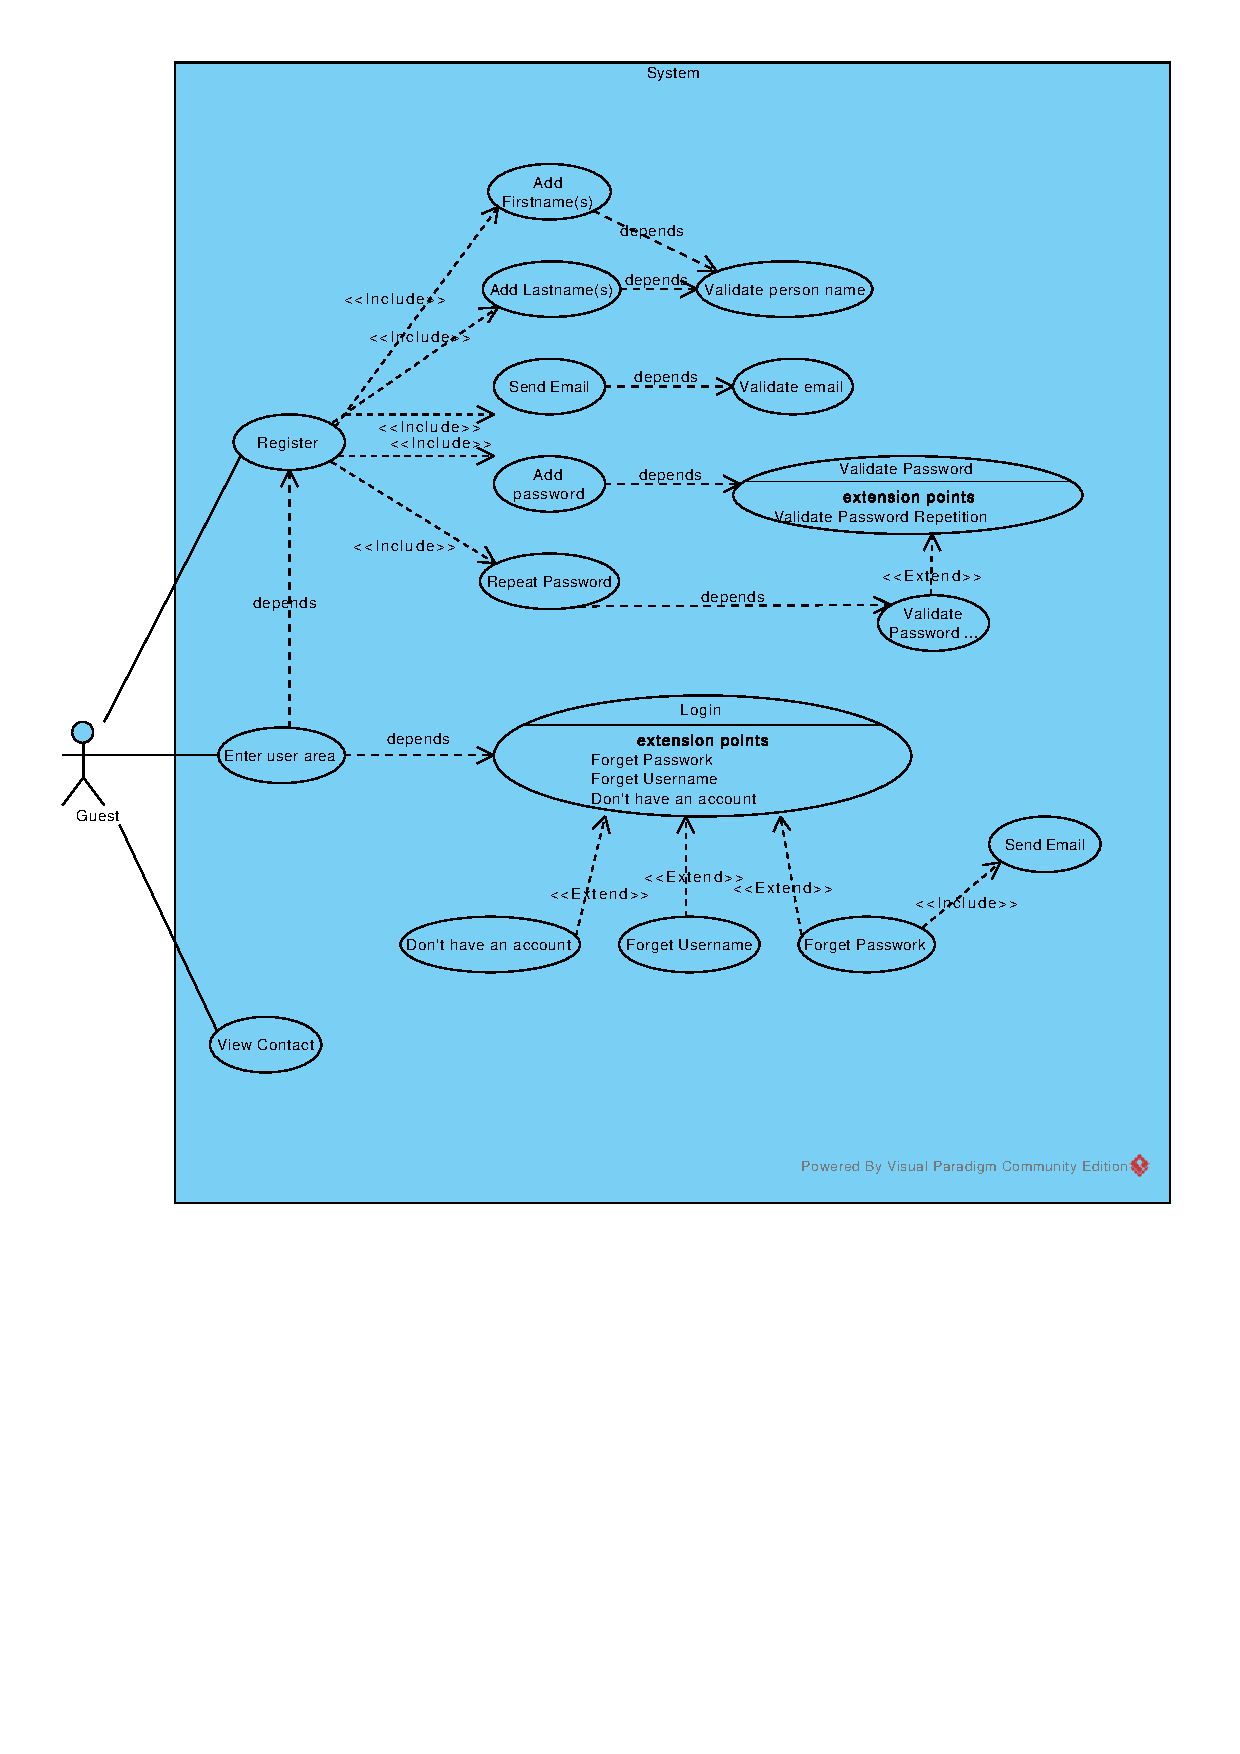
\includegraphics[scale=0.55]{figures/startup-use-case.pdf}
  \caption{Startup Use Case Diagram}
  \label{fig:startup-use-case}
\end{figure}
%
The startup use case \textbf{includes} the following use cases:
%

\begin{use-case}[Register]
  This use case is the only way to non-previleged become previleged
  users. The register use case consists on gathering minimal user data
  to create an account in the system. These data must be validated
  against predefined business constraints.
  \begin{sub-use-case}[Add first names]
    \label{uc:add-first-name}
    Users input their firstnames.
  \end{sub-use-case}
  \begin{sub-use-case}[Add last names]
    \label{uc:add-last-name}
    Users input their last names.
  \end{sub-use-case}
%
  \begin{sub-use-case}[Add email]
    \label{uc:add-email}
    Users input their email.
  \end{sub-use-case}
%
  \begin{sub-use-case}[Add password]
    \label{uc:add-password}
    Users input their password.
  \end{sub-use-case}
%
  \begin{sub-use-case}[Repeat password]
    \label{uc:repeat-password}
    User input their password a second time.
  \end{sub-use-case}
%
  \begin{sub-use-case}[Confirm data]
    \label{uc:condirm-data}
    User sends registration data.
  \end{sub-use-case}
%
  \begin{sub-use-case}[Clear data]
    \label{uc:clear-data}
    User clears registration data.
  \end{sub-use-case}
%
  \begin{sub-use-case}[Cancel]
    \label{uc:cancel}
    User cancel the registration process.
  \end{sub-use-case}
%
  \begin{sub-use-case}[Validate person name]
    \label{uc:add-first-name}
    Validates a person name.
  \end{sub-use-case}
%
  \begin{sub-use-case}[Validate email]
    \label{uc:add-email}
    Users input their email.
  \end{sub-use-case}
%
  \begin{sub-use-case}[Validate password]
    \label{uc:add-password}
    Users input their password.
  \end{sub-use-case}
%
  \begin{sub-use-case}[Validate password repetition]
    \label{uc:repeat-password}
    User input their password a second time.
  \end{sub-use-case}
%
  \begin{sub-use-case}[Validate]
    \label{uc:condirm-data}
    User sends registration data.
  \end{sub-use-case}
%
  \begin{sub-use-case}[Clear data]
    \label{uc:clear-data}
    User clears registration data.
  \end{sub-use-case}
%

\end{use-case}
%

%
\begin{use-case}[Enter User Area]
  \label{uc:enter-user-area}
  Access to \lifetime's previleged services for private clients. It
  depends on the login use case and it's extensions:
  \begin{sub-use-case}[Login]
  \end{sub-use-case}
  \begin{sub-use-case}[Forgot username]
  \end{sub-use-case}
  \begin{sub-use-case}[Forgot password]
  \end{sub-use-case}
  \begin{sub-use-case}[Don't have an account]
  \end{sub-use-case}
\end{use-case}
%
\begin{use-case}[View Contact]
  \label{uc:view-contact}
  For any visitor, gust or previleged, to access corporative, legal
  and communication services.
  \begin{sub-use-case}[Kontakt]
  \end{sub-use-case}
  \begin{sub-use-case}[Impressum]
  \end{sub-use-case}
\end{use-case}
%

\subsection{Class Diagram}
\label{sec:registation-class-diagram}
%



\subsection{Activity Diagram}
\label{sec:registation-activity-diagram}

%
\subsection{Tests}
\label{sec:tests}

\begin{test}[Test App Location]
  Test that the application is running in the expected location
\end{test}
\begin{test}[Test Security Context]
  Test that the application welcome page allows access to all kind of
  users.
\end{test}
\begin{test}[Welcome Services]
  Test that the welcome page has the following services:
  \begin{enumerate}
  \item Registration process to welcome new previleged users
  \item User Private Area, where previleged services are made
    available to users
  \item Contact page and formular, with \lifetime's corporative
    information.
  \end{enumerate}
\end{test}
\begin{todo}[Change location]
  Address should be http://localhost/lifetime
\end{todo}













\section{User Services}
\label{sec:user-use-services}
Users services are made available after successful login. Login
dynamically changes the a visitor's role from guest to previleged
user. For loged in users \lifetime offers the services described in
the section \ref{sec:user-use-cases}.

\subsection{Requirements}
\label{sec:user-requirements}

\subsection{Use Cases}
\label{sec:user-use-cases}
The use case diagram for accessing user services is depicted in
Figure~\ref{fig:user-use-cases}, featuring use cases below.
%
\begin{figure}[htpb]
  \centering
  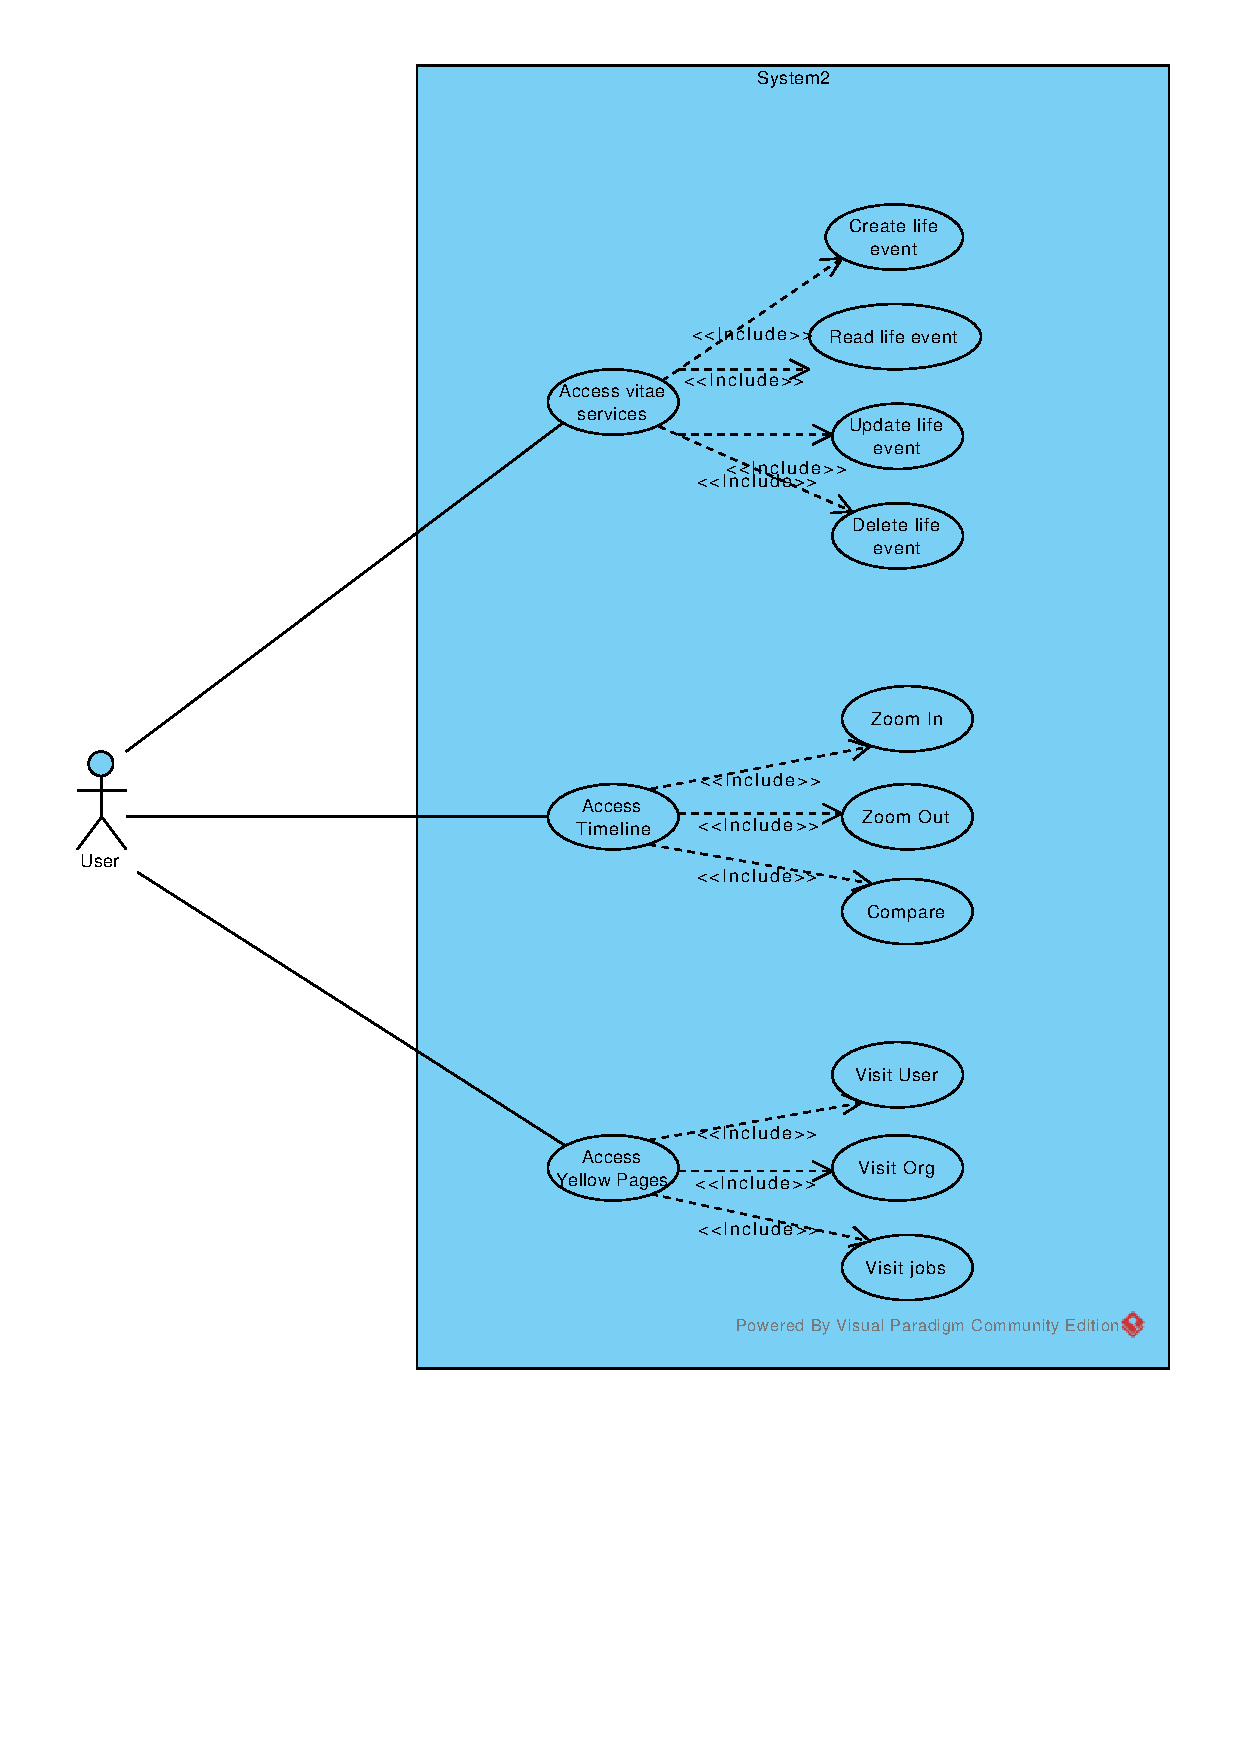
\includegraphics[scale=0.55]{figures/user-use-cases.pdf}
  \caption{User use case diagram}
  \label{fig:user-use-cases}
\end{figure}
%

%
\begin{use-case}[Access \vitae services]
  
\end{use-case}
\begin{use-case}[Access \timeline services]
  
\end{use-case}
\begin{use-case}[Access \yellowpages services]
  
\end{use-case}

\subsection{Class Diagram}
\label{sec:user-class-diagram}


\subsection{Activity Diagram}
\label{sec:user-activity-diagram}

\subsection{Tests}
\label{sec:user-tests}





\section{Administration Services}
\label{sec:admin-use-cases}
\subsection{Requirements}
\label{sec:user-requirements}

\subsection{Use Cases}
\label{sec:admin-use-cases}

\subsection{Class Diagram}
\label{sec:admin-class-diagram}


\subsection{Activity Diagram}
\label{sec:admin-activity-diagram}

\subsection{Tests}
\label{sec:admin-tests}


%%% Local Variables:
%%% mode: latex
%%% TeX-master: "main"
%%% End:
